
\section{Questions, hypotheses and findings}

The questionnaire starts with recalling the European debt
crisis that began in 2010, and the memoranda of understanding
that Greece, Spain, Portugal, Ireland and Cyprus signed with the European
Union, the European Central Bank and the International Monetary Fund that  
established financial aid combined with economic adjustment. We refer to
these contracts as \textit{aid\&reform} programs. 
We investigate whether country
origin matters for respondents' opinions about the reasons for why lender countries wanted to engage in the credit relationship. 
\begin{figure}[h!]
\caption{Reasons of the lender countries for entering the rescue program}
    \begin{center}
    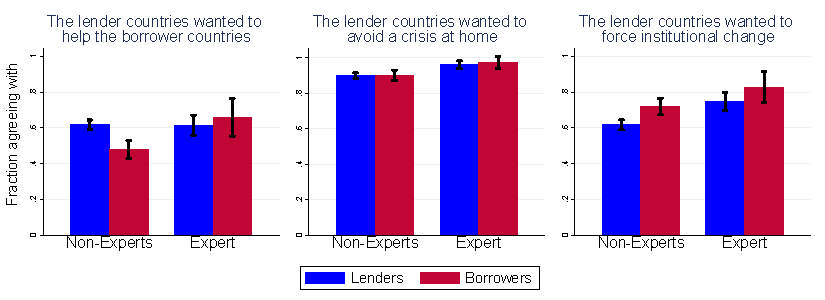
\includegraphics[scale=1.2]{graph2.pdf}
    \label{fig:Figure1}
    \end{center}
     \tiny
     \begin{tablenotes} 
    {The exact wording of the question is: In your opinion, what is the main reason why these countries entered these programmes 2a The lender countries wanted to help the borrower countries; 2b The lender countries wanted to help themselves to avoid a major crisis at home; 2c The lender countries wanted to force their desire for institutional change upon the borrower countries. Participants could choose the options strongly agree, slightly agree, slightly disagree and I don't know. We exclude all participants who answered with I don't know.\\
    The whiskers represent the 95 \% confidence intervals}
    \end{tablenotes}
\end{figure}

The nation-serving hypothesis is:\ respondents from borrower countries tend
to agree less frequently than respondents from lender countries 
that the lender countries wanted to help. They agree more that
the lender countries wanted to help themselves, and they agree more 
often that the lender countries wanted to force institutional change on the
crisis countries.\textit{\ }

The nation-serving hypothesis is not rejected based on our data (\autoref{fig:Figure1}). The share of non-experts from lender countries agreeing that lender countries wanted to help the borrower countries (62\%) is larger than the share of non-experts from borrower countries (48\%).
The difference in assessments between
non-experts from borrower and lender countries are large and statistically
significant at the 1 \% level for this aspect of the reforms. There is also some disagreement in the expert sample. The differences, however, do not turn out to be statistically significant. \\
It is conceivable that
many non-expert respondents in the borrower countries believe that
the lender countries had an institutional-reform agenda that goes beyond the
idea of helping each other. Participants from borrower and lender countries agree that lender countries wanted to avoid a crisis at home both in the expert and non-expert sample. The nation-serving bias manifests itself again in the non-expert sample in the question about the desire for institutional change among the lender countries. 62 \% of non-experts from lender countries agree with this statement compared to 72 \% among the lender countries. Again, we observe differences in answers among the expert sample as well which do not turn out to be statistically significant. 
It is conceivable that experts, apart from simply being
better informed, often identify less with their own countries of origin and have 
a more cosmopolitan orientation. Therefore, the
forces for developing a nation-bias might be less strong for experts than for non-experts. 

\begin{figure}
    \begin{center}
      \caption{Driving Force and Beneficiaries}
    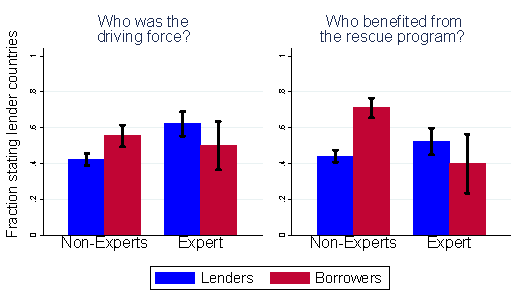
\includegraphics[scale=1.2]{graph3.pdf}
  
    \label{fig:figure2}
    \end{center}
    \tiny
    \begin{tablenotes} 
    {The exact wording of the questions is: 3. In formal terms, the borrower countries that signed a memorandum had to apply for support. But thinking about the true motivations and the political processes behind these events, which of the following three alternatives corresponds most closely to your perceptions. Answer options: The borrower countries wanted it, the lender countries were more reluctant; The lender countries wanted it, the borrower countries were more reluctant; Both wanted it equally; I don't know \\
   Question 4: Who do you think mainly benefited from the rescue program. Answer options: The borrower countries; The lender countries; Both groups of countries benefited equally; I don't know. We exclude all participants who answered with I don't know. \\
   The whiskers represent the 95 \% confidence intervals.}  
    \end{tablenotes}
\end{figure}
The following questions corroborate that the difference in nation-serving bias is a more systematic pattern (\autoref{fig:Figure1}). They show very similar patterns for non-expert
respondents, depending on whether they are from borrower countries or from
lender countries. The results suggest large and significant nation-biases. Question 3 is similar to Question 2 and asks the respondents about the driving force behind the \textit{aid\&reform programs}. Question 4 asks about the main beneficiaries of the aid&reform program. Non-experts
from borrower countries tend to see the lender countries as the main
motivators for these programs. This result corroborates the results on
self-serving memories from private informal lending as in \cite{dezso}, who report a tendency to assign the initiative\
for such contracts to the other side of the credit relationship. 

Non-experts from borrower and lending countries also differ in
their perceptions of who mainly benefited from the \textit{aid\&reform programs}. The
bias tends to assign the benefits more to the counterparty group:\
respondents from borrower countries think more often than respondents from
lender countries that the lender countries are the major beneficiaries. 

The responses of experts do not seem to be prone to a country-group
bias. Whether an expert is originally from a borrower country or a lender
country does not affect their assessments about the
motivations driving the \textit{aid\&reform programs}, nor their assessments about
who was the main beneficiary.\footnote{98 percent of experts also works in their country of origin }  Interestingly, there is a nation-disfavoring bias in the sample of experts. Experts from lender countries are 12 percentage points more likely to agree that lender countries were the driving force and the main beneficiaries of the rescue program (\autoref{fig:figure2}). However, these differences do not turn out to be statistically significant.

We now turn to questions addressing how the groups of respondents
assess the implications of the \textit{aid\&reform programs} for feelings among the
populations in the borrower and the lender
countries. The respondents' perceptions might be formed by direct
observations in the countries or media reports, but their views about the
reasons and motivations for the \textit{aid\&reform programs} and their views about
who actually benefited from these programs should correlate with their
assessments, and might cause their beliefs about these feelings. 

We ask whether respondents think that the rescue experience might
have caused feelings of \textit{guilt}, feelings of \textit{being
exploited}, and/or feelings of \textit{inferiority}. These questions do not directly reflect a nation-serving bias but might rather be the outcome of such a bias. For example, a respondent from Greece might think that the \textit{aid\&reform programs} mainly benefited the lender countries which forced Greece to undertake the reforms. Hence, a Greek respondent might not feel guilty due to the \textit{aid\&reform programs}. On the other hand, a respondent from the lender countries might feel that the \textit{aid\&reform programs} was a benevolent gesture from the lender countries which provided large benefits to the program countries. Hence, a respondent from the lender countries might be more prone to assume that citizens in the borrower countries felt guilt due to the large benefits they received.\footnote{Our findings can also be interpreted in an alternative way.  Having a self-serving or nation-serving bias might make individuals oblivious to
the way policies are received in other countries. 
\cite{dezso} refer to this phenomenon as having a ``blind spot" regarding the other party's 
feelings and emotions. The hypothesis on the existence of such a ``blind spot" is confirmed in our findings.
Citizens from lender countries are more likely to agree that they felt guilty, exploited and/or inferior as a 
consequence of the \textit{aid\&reform programs}. The largest difference between lender and borrower countries occurs with regards to feeling exploited.
78 percent  of citizens from borrower countries state that they felt exploited due to the \textit{aid\&reform programs} while only 61 percent of lender countries
agree to this statement. 
}

%Similar reasons might let us suspect that the respondents from the lender
%countries are more inclined to think their population feels exploited, or
%feel inferior (in the sense of humiliated). Figure xxx shows the answers.
%First statistics negate the existence of a blind spot among borrowers about the feelings
%from citizens to lender countries. 

\begin{figure}
\begin{center}
    \caption{Emotions of the borrower countries}
    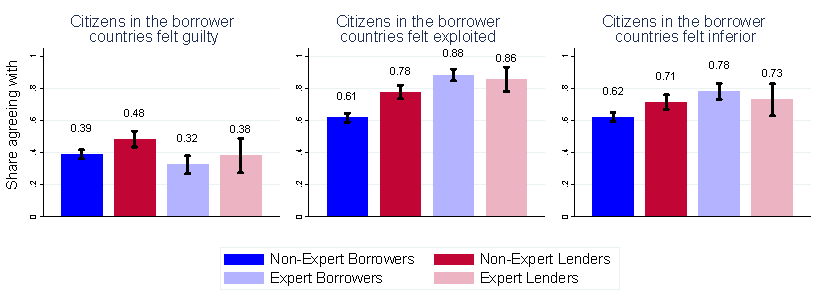
\includegraphics[scale=1.2]{graph5_1.pdf}
    \label{fig:figure3}
    \end{center}
    \tiny 
      \begin{tablenotes} 
      {The exact wording of the question was the following: Please give assessments of the following questions: 5a) The rescue experience made many citizens in the borrower countries feel guilty 
      5b) The rescue experience made many citizens in the borrower countries feel exploited 5c) The rescue experience mad many citizens in the borrower countries feel inferior
      Answer options: strongly agree, slightly agree, slightly disagree, strongly disagree, I don't know. We exclude all participants who answered with I don't know. \\
      The whiskers represent the 95 \% confidence intervals.}
      \end{tablenotes}
\end{figure}

As expected the view of experts is not influenced by their countries of origin.  (\autoref{fig:figure3}).


Similar questions assess the perceptions in the groups about the
feelings in the lender countries. In particular, we asked the participants whether they
agree that the \textit{aid\&reform programs} made the citizens in the
lender countries feel exploited and disappointed (\autoref{fig:figure4}). Differences in the answers to these questions might manifest themselves as a consequence of  a nation-serving bias. If citizens from lender countries feel that the borrower countries were the driving force behind the \textit{aid\&reform programs} and also the party which reaped the highest benefit from these programs, they might report to feel exploited. If borrower countries feel they did not benefit from the program and also did not initiate the program, they will infer that lender countries should have no reason to feel guilty. Overall, we might expect that the lender-country respondents agree more
frequently than the borrower-country respondents to the possibly negative
feelings in lender countries.

\begin{figure}[h!]
  \begin{center}
       \caption{Emotions of the lender countries}
    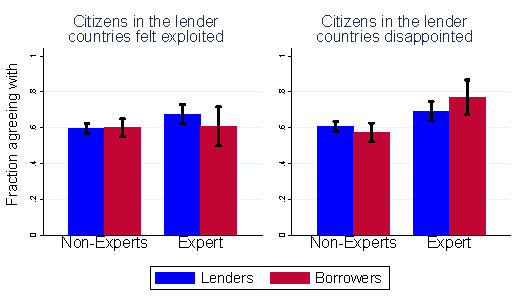
\includegraphics[scale=1.2]{graph5_2.pdf}
 
    \label{fig:figure4}
    \end{center}
    \tiny
    \begin{tablenotes}
     {The exact wording of the question is: 5d) The rescue experience made many citizens in the lender countries feel exploited 5e) The rescue experience made many citizens in the lender countries feel disappointed
    Answer options: strongly agree, slightly agree, slightly disagree, strongly disagree, I don't know. We exclude all participants who answered with I don't know. \\
    The whiskers represent the 95 \% confidence intervals}
    \end{tablenotes}
\end{figure}

The results do not suggest that respondents from borrower countries have different views than respondents from lender countries. The findings indicate that the respondents
in both groups of countries believe that the \textit{aid\&reform programs} triggered
negative feelings in both groups of countries. A large share of the respondents
thinks that citizens in borrower countries feel guilty, exploited, and
inferior, and a large share of respondents also thinks that citizens in
lender countries feel disappointed and exploited as well. 

We also ask whether the \textit{aid\&reform programs} strengthened friendship between the citizens in the Eurozone. The theory of groups and conflicts shows that, when groups jointly master a major task which none of them could have mastered alone, they overcome negative attitudes and mutual spite between groups HABEN WIR HIERZU REFERENZEN ZUM ZITIEREN?. The European debt crisis had the potential to be 
such a task. It might have strengthened friendship between these groups.
However, if both groups have nation-serving biases about what
motivated the crisis and the solution method adopted, and about the
distribution of the benefits and costs of the method adopted, then we might
expect that a large fraction of the respondents of both groups think that
these programs did not strengthen friendship ties. 
\begin{figure}
\begin{center}
\caption{Impact on friendships}
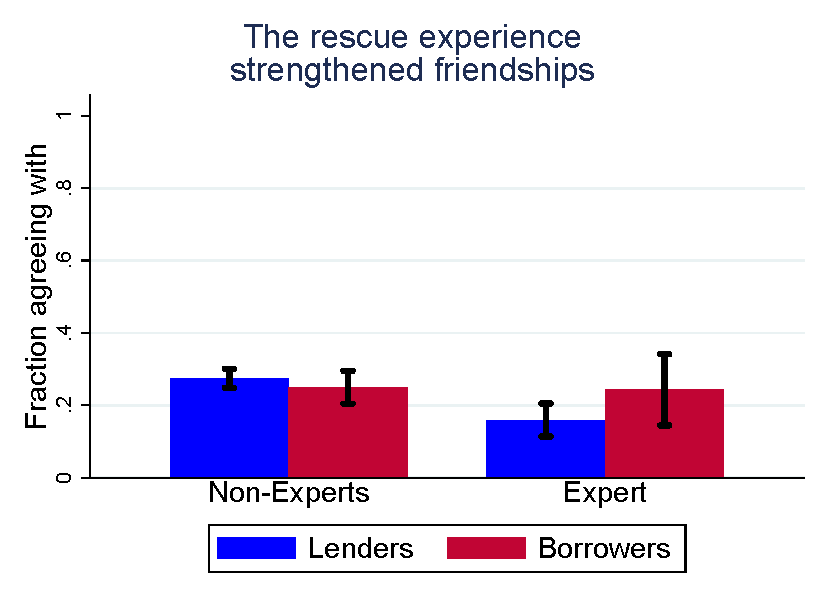
\includegraphics[scale=0.5]{graph5_3.pdf}
\label{fig:figure5}
\end{center}
\tiny 
\begin{tablenotes}
  {The exact wording of the question is the following: 5f) The rescue experience strengthened friendships
   Answer options: strongly agree, slightly agree, slightly disagree, strongly disagree, I don't know. We exclude all participants who answered with I don't know. \\
     The whiskers represent the 95 \% confidence intervals}
    \end{tablenotes}
\end{figure}

The majority of participants from the expert and non-expert sample disagrees that 
the rescue package strengthened friendships (\autoref{fig:figure5}).\footnote{Due to a survey error this question was displayed as "The rescue experience strengthened friendship ties between borrower". The fraction of experts who answered this question with "I don't know" lies around 20 percent. This is very much in line with the frequency of "I don't know" responses throughout the survey. Hence, it seems plausible that participants correctly understood the question. } This holds for participants from 
both the expert and the non-expert sample. This finding suggests that non-experts are aware of the divergence of views between lender and borrower countries and tensions arising from such divergences. In light of the absence of such a bias among the expert sample 
it seems interesting that the level of agreement in this sample is also quite low. 
This might suggest that although experts might not have and be aware of a nation-serving bias
among citizens from the lender countries they are indeed aware of the consequences of such 
a nation-serving bias. 


The reasoning that discussed possible hypotheses for the answers to
questions 5a-5e suggests that answers to the various questions are likely to
be interdependent. We might expect that individuals in lender countries who
think that the borrower countries pushed for the aid\&reform programs
(questions 2 and 3) also think that these are the main beneficiaries
(question 3), and therefore think that the lender countries feel exploited
and disappointed. The direction of causality for respondents from the lender
countries would be%
\begin{equation*}
\begin{array}{ccccc}
\begin{array}{c}
\text{borrower countries} \\ 
\text{pushed for aid\&reform}%
\end{array}
& \rightarrow  & 
\begin{array}{c}
\text{borrower countries} \\ 
\text{are the main} \\ 
\text{beneficiaries of} \\ 
\text{aid\&reform}%
\end{array}
& \rightarrow  & 
\begin{array}{c}
\text{lender countries} \\ 
\text{feel exploited} \\ 
\text{and disappointed.}%
\end{array}%
 \end{array}%
 \end{equation*}


 We evaluate this chain of causality empirically: 
 \begin{table}[h!]
     \centering
     \begin{tabular}{c|c}
          &  \\
          & 
     \end{tabular}
     \caption{Chain of Causality I}
     \label{tab:my_label}
 \end{table}
 \begin{table}[h!]
   \centering
    \begin{tabular}{l*{1}{}
    \hline\hline
    &Participants who believe that borrowers were the main driving force of the program & Participants who believe that lender countries or both countries equally were the main driving force of the program \\
    \hline
Share agreeing that the borrowers benefited from the rescue program&0.47&0.24\\
Share agreeing that the lenders felt exploited&0.59&0.61\\
Share agreeing that the lenders felt disappointed&0.65&0.63\\
\hline\hline
    
    \end{tabular}
   \end{table}

 \begin{table}[h!]
   \centering
 \begin{tabular}{l*{1}{cc}}
 \hline\hline
                     &\multicolumn{2}{c}{}     \\
                       &Lenders felt exploited&  Lenders felt disappointed\\
 \hline
 Borrowers did not benefit                   &        0.59&        0.60\\
 Borrowers benefited                   &        0.65&        0.65\\
 Total               &        0.61&        0.62\\
 \hline\hline
 \end{tabular}
 \begin{tablenotes}
  \small
 \item The table depicts conditional correlations. We show the share of participants agreeing with the statements conditional on their answer to question 4: Who benefited from the rescue program?
 \end{tablenotes}
 \end{table}



 We find that this correlation only works partially. Participants who agree with the statement that the borrower (lender) countries were the driving force behind the reform are also more likely to agree that the borrower (lender) countries were the main beneficiaries of the aid& reform package. The assessment of which party was the driving force does not influence participants opinions on the feelings that were evoked among borrower or lender countries. However, participants who agree with the statement that the lender countries were the main beneficiaries from the rescue program also show a higher likelihood to agree that the borrower countries felt guilty/ exploited or inferior due to the rescue program. For participants who agree that the 
 Respondents from the borrower countries who think that the lender countries
 pushed for the aid\&reform programs, wanted to impose institutional reforms
 on them are probably the same who think that the lender countries are the
main beneficiaries, and also the same ones who think that the borrower
countries have been exploited and would not feel guilt, but feel humiliated
("inferiority"?). The direction of causality is%
\begin{equation*}
\begin{array}{ccccc}
\begin{array}{c}
\text{lender countries} \\ 
\text{pushed for aid\&reform} \\ 
\text{and wanted to impose} \\ 
\text{structural reforms}%
\end{array}
& \rightarrow  & 
\begin{array}{c}
\text{lender countries} \\ 
\text{are the main} \\ 
\text{beneficiaries of} \\ 
\text{aid\&reform}%
\end{array}
& \rightarrow  & 
\begin{array}{c}
\text{borrower countries} \\ 
\text{feel exploited}%
 \end{array}%
 \end{array}%
 \end{equation*}
  \begin{table}[h!]

 \centering
 \caption{Chain of Causality II}
 \resizebox{1.1\textwidth}{!}{%
   \hskip -2.0cm
 \begin{tabular}{l*{1}{cccc}}
 \hline\hline
                     &\multicolumn{4}{c}{}                               \\
                     &  Lenders benefited & Borrowers felt guilty &  Borrowers felt exploited & Borrowers felt inferior\\
 \hline
 Lenders were not driving force                 &        0.32&        0.40&        0.63&        0.65\\
 Lenders were driving force                &        0.70&        0.40&        0.78&        0.72\\
 Total               &        0.51&        0.40&        0.70&        0.68\\
 \hline\hline
 \end{tabular} }
  \begin{tablenotes} 
 \small
  \item The table depicts conditional correlations. We show the share of participants agreeing with the statements conditional on their answer to question 3: Who was the driving force?
 \end{tablenotes}
 \end{table}

 \begin{table}[h!]
    \centering
 \begin{tabular}{l*{1}{ccc}}
 \hline\hline
                     &\multicolumn{3}{c}{}                  \\
                     &  Borrowers felt guilty &  Borrowers felt exploited & Borrowers felt inferior\\
 \hline
 Lenders did not benefit                  &        0.35&        0.58&        0.58\\
 Lenders benefited                 &        0.45&        0.81&        0.74\\
 Total               &        0.40&        0.70&        0.66\\
 \hline\hline
 \end{tabular}
   \begin{tablenotes} 
 \small
 \item The table depicts conditional correlations. We show the share of participants agreeing with the statements conditional on their answer to question 4: Who benefited from the rescue program?
\end{tablenotes}
 \end{table}
 
 \clearpage
 In addition we also run inter country comparisons of answers for the non-expert sample. Due to the small size of our expert sample we refrain from running inter-country comparisons. 


  \begin{table}[h!]
 \caption{ Comparison of Means between individual program country and sample means} 
 \resizebox{\textwidth}{!}{%
 \begin{tabular}{*{7}{>{\centering\arraybackslash}p{.13\linewidth}}}
 \hline\hline
 &\multicolumn{4}{c}{\textbf{Deviation from the Program Country Mean}} &\multicolumn{2}{c}{\textbf{Means}} \\
            Question &\multicolumn{1}{c}{Greece}&\multicolumn{1}{c}{Ireland}&\multicolumn{1}{c}{Portugal}&\multicolumn{1}{c}{Spain}&\multicolumn{1}{c}{Program (mean)}&\multicolumn{1}{c}{Non-Program (mean) }\\

 \hline
2.1 (-)       &       -0.20&        0.11&       -0.04&        0.03&        0.51&        0.62\\
 2.2 (+)        &        0.05&        0.01&       -0.03&       -0.06&        0.91&        0.90\\
 2.3 (+)       &        0.13&       -0.19&        0.03&       -0.08&        0.74&        0.62\\
 \hline
 &&&&&& \\
5.1 (+)        &        0.11&        0.04&       -0.05&       -0.02&        0.47&        0.39\\
5.2 (+)        &        0.14&       -0.05&       -0.01&       -0.16&        0.79&        0.61\\
5.3 (+)        &        0.10&        0.03&       -0.10&       -0.04&        0.72&        0.62\\
5.4 (-)        &        0.13&       -0.10&       -0.03&       -0.04&        0.60&        0.60\\
5.5 (-)        &        0.08&       -0.18&       -0.03&       -0.04&        0.61&        0.61\\
5.6  ()       &       -0.14&        0.10&        0.05&        0.02&        0.25&        0.27\\
 \hline
 &&&&&& \\
 6  (+)         &        0.04&       -0.02&       -0.02&        0.03&        0.32&        0.18\\
 3  (+)          &        0.14&        0.03&       -0.12&       -0.03&        0.54&        0.43\\
 4  (+)          &        0.17&        0.03&        0.05&       -0.17&        0.67&        0.44\\
 7  (+)          &        0.31&       -0.11&       -0.06&       -0.12&        0.55&        0.36\\
 \hline\hline

 \end{tabular} }
 \begin{tablenotes}
 \footnotesize
 \item The sign in parantheses denotes the expectation about the difference in assessments between program and non-program countries. The left-hand side illustrates the difference between single program countries and the overall program country mean. The right hand side shows the program country mean and the non-program country mean. 
 \end{tablenotes}
 \end{table}
 
 